\documentclass[a4paper,10pt]{article}

\usepackage[utf8]{inputenc}
\usepackage{mathtools}
\usepackage{amsfonts}
\usepackage{amsmath}


\title{\textbf{Computer Graphics} \\ Assignment 4}
\author{Thierry CANTENOT \\ J114030901}
\date{07/05/15}

\pdfinfo{%
  /Title    (Assignment 4)
  /Author   (Thierry CANTENOT)
  /Creator  ()
  /Producer ()
  /Subject  (Computer Graphics)
  /Keywords ()
}

\begin{document}
\maketitle

\section{Space partitionning}
\bigskip

\subsection{BSP}
\bigskip

\subsubsection{Problem statement}
\bigskip

Generate a M shaped BSP tree.

\subsubsection{Answer}
\bigskip

Let consider the following M shaped polygons.

    \begin{figure}[!htb]\centering

            \frame{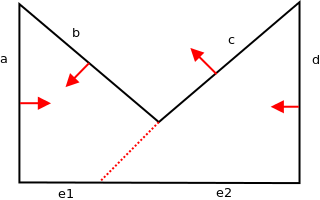
\includegraphics[width=0.6\linewidth]{./images/m.png}}
            \caption{M-shaped polygon}
    \end{figure}

\noindent
First let split the polygon along the $c$ edge: this split the $e$ edge in two. \\
Then on the positive side we split along $b$: the positive side contains $a$ and $e1$, the negative side nothing. \\
Then on the positive side of $b$ we split along $a$: the positive side contains $e1$, the negative side nothing. \\
Then we go back to $c$, consider its negative side containing $d$ and $e2$ and split along $d$: the positive side contains $e2$, the negative side nothing. \\
And then we are done, the resulting BSP tree is as follow:

 \begin{figure}[!htb]\centering
        \frame{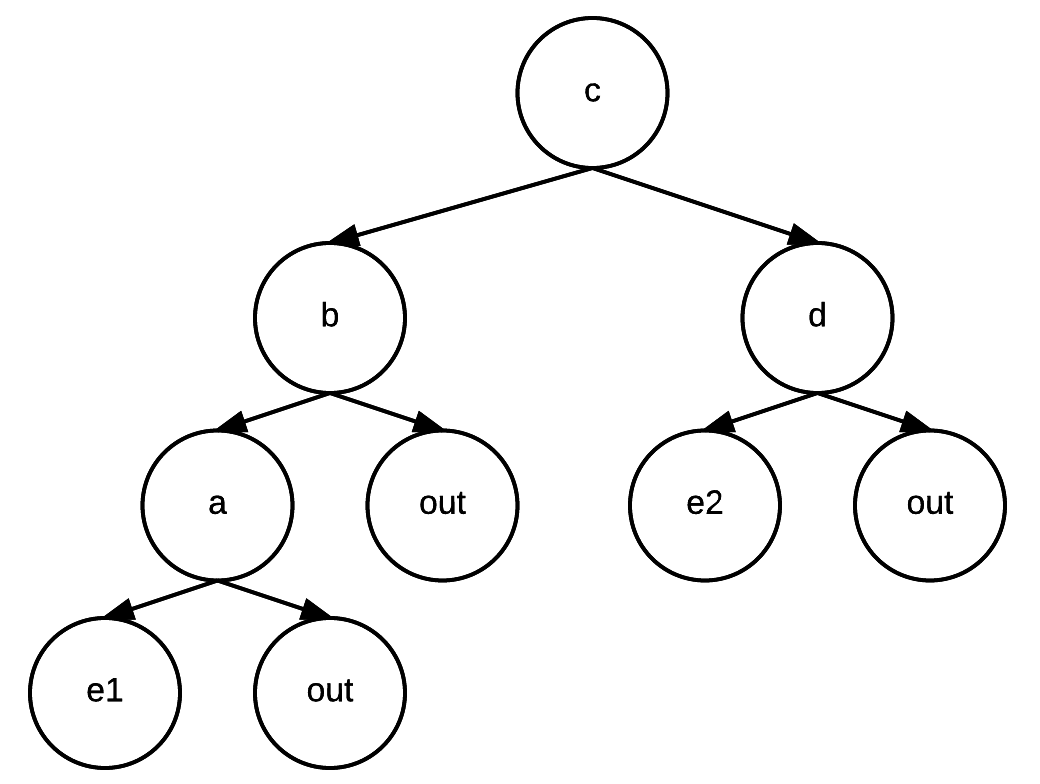
\includegraphics[width=0.7\linewidth]{./images/bsp.png}}
        \caption{BSP tree}

    \end{figure}  

\end{document}
